\chapter {Dice game}
\section{Project description}

The purpose of the second project was to analyse die rolls for the purpose of playing a popular dice game called ``Yahtzee''. The game consists of rolling 5 dies a maximum of 3 times per turn. Desirable rolls are kept aside and the remainder is cast again. The objective is to score as many points as possible by placing the final rolls in one of 15 categories. 

In particular, it was attempted to be able to read off the die rolls with a single camera. A number of existing methods were found which utilised multiple cameras to increase the accuracy of the readings \cite{hsu2012color}, for example in widely varying lighting conditions. As the lighting conditions could be controlled in this project, only a single camera was chosen. 

Additionally, two constraints were added. First, the camera is allowed to be positioned at skew angles, and not directly above the scene. Second, the size of the dies is not given. This is in effect similar to allowing the camera to be placed at different heights.

\section{Method}
\subsection{Overview}
The general methodology that was adopted for extracting the die rolls from the image taken by the camera was as follows:
\begin{enumerate}
\item Segment the image into areas that might represent dots and background pixels.
\item Deduce which of those areas actually represent dots.
\item Deduce which dots belong to the same die face.
\end{enumerate}

Each of these steps will be discussed and supported in detail.

The project uses a set of standard dice. In particular, white dies with black dots. For the remainder of this report, whenever a feature of a die is mentioned it is considered a feature most dice in existence posess.

\subsection{Image segmentation step}
The objective of this step is to obtain a binary image which solely contains information related to dots so that inforation about them can be extracted in the subsequent step. The aforementioned high-contrast colouring of standard dice is a very useful feature for segmentation as it is relatively easy to exploit.

\subsubsection{Problems which complicate segmentation}
Unfortunately, dice also exhibit some features which significantly complicate the segmentation process:

\begin{description}
\item[Rounded off corners] In order to encourage dice to roll before finally landing on a surface the corners and edges of dice are rounded off. This significantly complicates the detection process of die faces, as colours change gradually rather than instantly from one side to the next. This makes it much harder to find out which face a detected dot belongs to. Figure \ref{fig:diesEdges} shows a die together with an object with sharp corners. It is easier to extract data about different surfaces on the object with sharp corners because the rapid changes in colour can be exploited. In the case of dice this is much more difficult.

\begin{figure}
	\centering
	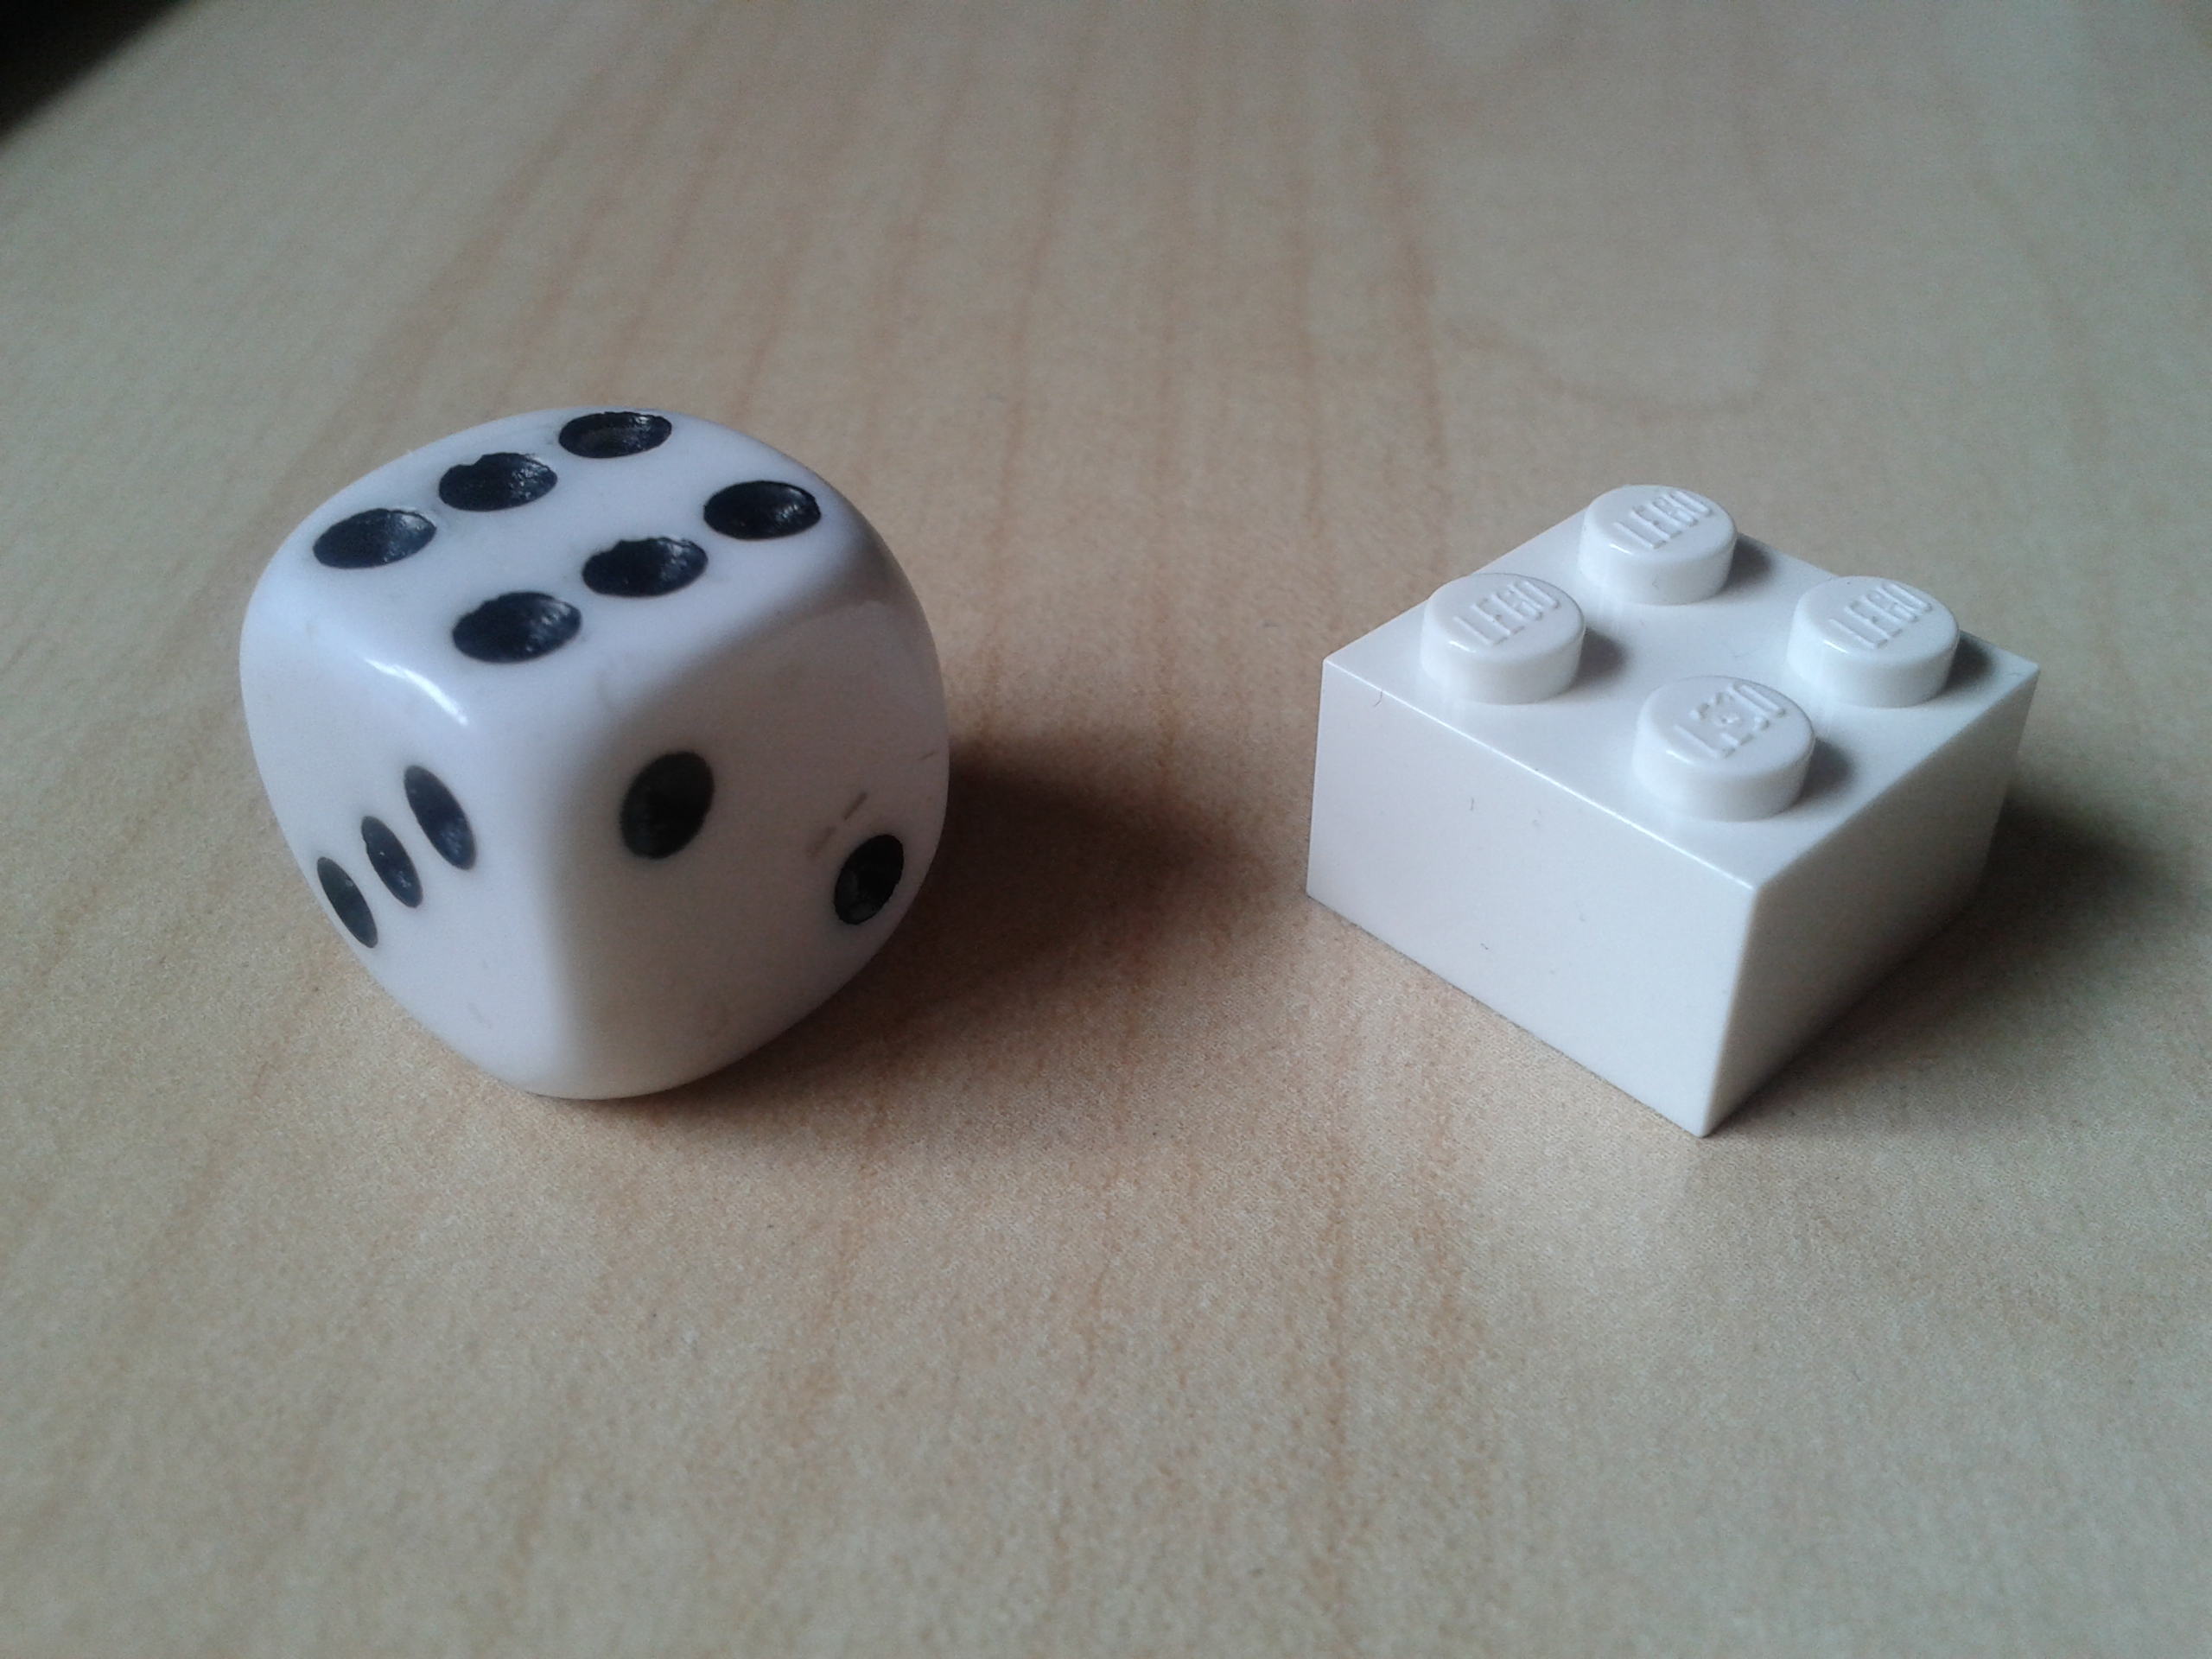
\includegraphics[width=50mm]{images/dies/edges.jpg}
	\caption{A single die and a shape with sharp edges.}
	\label{fig:diesEdges}
\end{figure}

\item[High specular factor] Dice are commonly polished. This surface therefore has a high specular factor which in turn results in many specular reflections that are picked up by the camera. 
\item[Dots are not flat] To allow blind people to read off their die rolls, the dots on dies are slightly hollowed out. Due to their shape an additional specular reflection is created on each dot. On this image this is represented as a much lighter coloured area inside an area which should preferrably be black completely. Figure \ref{fig:dotSpecular} shows the effect such specular reflections can have. The segmented image clearly shows reduced performance because of the brighter colours inside the die dots.

\begin{figure}
	\centering
	\begin{subfigure}[b]{3cm}
		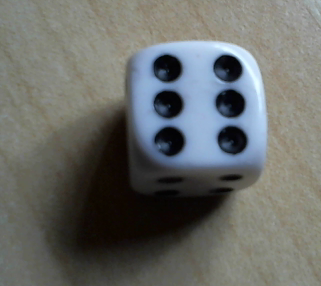
\includegraphics[width=30mm]{images/dies/specular.png}
		\caption{Original}
		\label{fig:dotSpecularOriginal}
	\end{subfigure}
	%
	\hspace{1cm}
	%
	\begin{subfigure}[b]{3cm}
		
\includegraphics[width=30mm]{images/dies/specular_thresholded.png}
		\caption{Segmented}
	\end{subfigure}

	\caption{A single die showing specular reflections within its dots, and the result of its segmentation.}
	\label{fig:dotSpecular}
\end{figure}

\item[Shadows] In figure \ref{fig:dotSpecularOriginal} can also be seen that shadows may contain shadows. These can be quite dark depending on the lighting conditions. They may thus be picked up by the segmentation algorithm as possible dots. 
\end{description}

\subsubsection{Developed method}
The method used in the final product is the following sequence of filters:

\begin{description}
\item[Gaussian blur (9x9 kernel)] Used to reduce the noise level going into the filtering process. The used camera showed significant amounts of noise in low-light conditions. Aplying a blur on beforehand significantly increased the quality of the dot recognition.

\begin{figure}
	\centering
	\begin{subfigure}[b]{45mm}
		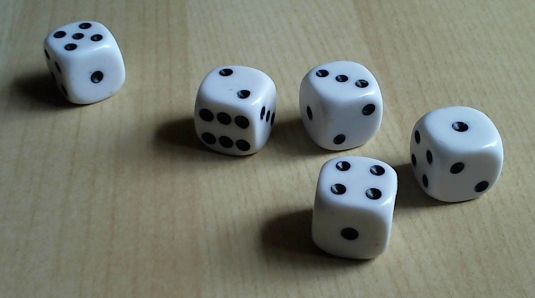
\includegraphics[width=45mm]{images/dies/original.png}
		\caption{Original}
	\end{subfigure}
	%
	\hspace{0.5cm}
	%
	\begin{subfigure}[b]{45mm}
		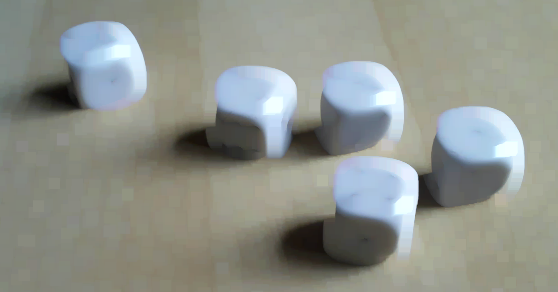
\includegraphics[width=45mm]{images/dies/dilated.png}
		\caption{Dilated}
	\end{subfigure}
	%
	\hspace{0.5cm}
	%
	\begin{subfigure}[b]{45mm}
		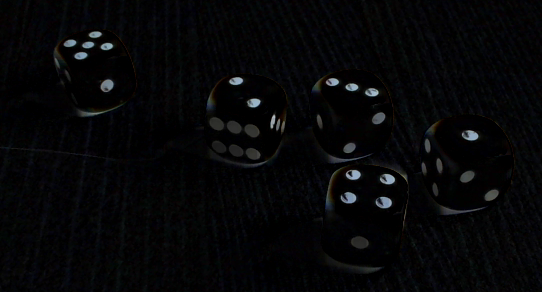
\includegraphics[width=45mm]{images/dies/difference.png}
		\caption{Difference}
		\label{fig:imgdiff}
	\end{subfigure}

	\caption{The bottom-hat filtering process.}
	\label{fig:bottomhat}
\end{figure}

\item[Bottom-Hat (11x11 square kernel)] Method from lecture 6, slide 42. This is the most important part of the filter sequence. Its main objective is to increase the contrast between the dice and the die faces while simultaniously reducing much of the background noise. The results of the individual processing steps are shown in figure \ref{fig:bottomhat}. The initial dilation causes the dots to disappear. Calculating the difference after an erosion step gives a nice segmentation of the dots as shown in figure \ref{fig:imgdiff}. The dots on the dice are clearly visible.

Also note that most of the sharp shadows have been taken out, as has the background which in itself was not a noise-free surface. However, some of the thinner shadows and darker surfaces have also come through.

The Bottom-Hat filter was chosen because of its ability to filter out high-contrast features on an image while simultaneously reducing background noise. A number of filters have been tried on this problem, though this method came out superior.

\item[Threshold (Otsu's method)] Finally, the image is converted into a binary image using a thresholding filter. The threshold level is determined using Otsu's method, as the image clearly contains two distinct sets of brighter and darker pixels. Otsu's method is also stronger in adapting to different lighting conditions as the intensity of the pixels from the original camera frame can vary. A single constant threshold was thus not satisfactory for this purpose.

\end{description}

\subsubsection{Attempted alternate methods}

\begin{figure}
	\centering
	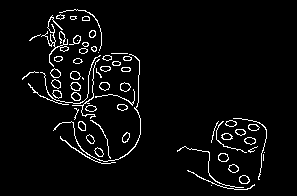
\includegraphics[width=40mm]{images/dies/canny_2.png}
	\caption{A canny edge detector applied on a captured image frame.}
	\label{fig:cannyEdge}
\end{figure}

\begin{description}
	\item[Canny edge detector] A more direct approach that was considered was to use a canny edge detector to locate the edge between a die dot and its background. Which is the followed up by a detector of ellipses to classify the individual dots. This method had some promising results, as shown in figure \ref{fig:cannyEdge}. However, the method described above was chosen in favour of it because it did not discard information about the location of darker patches while simultaniously being able to extract a similar boundary in its later stages. As this gave an overall higher information level, the edge detection method was not used.
	\item[Dynamic threshold] It was attempted to use a dynamic threshold in favour of a global one. In particular a gaussian threshold. This unfortunately only served as a means to amplify the background noise while simultaniously giving comparable results for the binarisation of dots to when Otsu's method was used.
\end{description}